% assignment_1.tex
% CS 8735 - Unsupervised Learning (Fall 2015)
%     University of Missouri-Columbia
%             Chanmann Lim
%            September 2015

\documentclass[a4paper]{article}

\usepackage[margin=1 in]{geometry}
\usepackage{listings}
\usepackage{amsmath}
\usepackage{graphicx}
\usepackage{float}

\everymath{\displaystyle}
\DeclareMathOperator*{\argmax}{\arg\!\max}

\begin{document}
\title{CS 8735: Report for assignment 1}
\author{Chanmann Lim}
\date{September 17, 2015}
\maketitle

\paragraph{Problem 1.} In this task, we are given a dataset generated from a mixture density and the job is to implement EM algorithm to learn the parameters of the model. Based on the assumption that the Gaussian Mixture Model has four component Gaussian PDFs with each having a full covariance matrix we will terminate the our EM estimation at the 100\textsuperscript{th} iterations. \\

\noindent The Matlab code for the experiment is in the \textbf{Appendix} section.

\paragraph{a) } For the first experiment which we named it case \textbf{a}, we run EM procedure with the initialization suggested in the assignment.

$$ \pi_k^{(0)} = 1/4 \qquad 1 \le k \le 4 $$
$$ \mu_1^{(0)} = [10\;2]^T, \mu_2^{(0)} = [5\;6]^T, \mu_3^{(0)} = [0\;1]^T, \mu_4^{(0)} = [4\;3]^T $$
$$ \Sigma_k^{(0)} = \mathbf{I}_{2\times2} \qquad 1 \le k \le 4 $$

After the EM procedure terminated, we got

\begin{equation}
	\hat{\pi}_1 = 0.3457, \hat{\pi}_2 = 0.1401, \hat{\pi}_3 = 0.1847, \hat{\pi}_4 = 0.3295\\
\end{equation}
\begin{align}
	\mathbf{\hat{U}} &= \begin{bmatrix}
							\hat{\mu}_1 & \hat{\mu}_2 & \hat{\mu}_3 & \hat{\mu}_4 
						\end{bmatrix} \\
					 & = \begin{bmatrix}
							13.0263  &  4.0619  &  1.6026  &  6.9183 \\
    						3.0455  &  7.9674  &  1.5717  &  5.9843
						 \end{bmatrix}
\end{align}
\begin{align}
	\mathbf{\hat{\Sigma}} &= \begin{bmatrix}
								\hat{\Sigma}_1 & \hat{\Sigma}_2 & \hat{\Sigma}_3 & \hat{\Sigma}_4 
							 \end{bmatrix} \\
						  & = \begin{bmatrix}
									1.6470  &  0.8788  &  8.4468  &  6.2731 \\
								   -0.7471  &  0.2342  & -0.0635  &  2.6295 \\
								    2.0688  &  1.1568  &  1.0938  &  1.9615
						 	  \end{bmatrix}
\end{align}

Where, $\hat{\Sigma_k}$ is the upper triangular values for covariance matrix of the $k^{th}$ Gaussian component. $$1 \le k \le 4$$

Figure ~\ref{fig:log_likelihood_a} shows that EM has converged at around the 80\textsuperscript{th} iteration.

\begin{figure}[H]
  \centering
    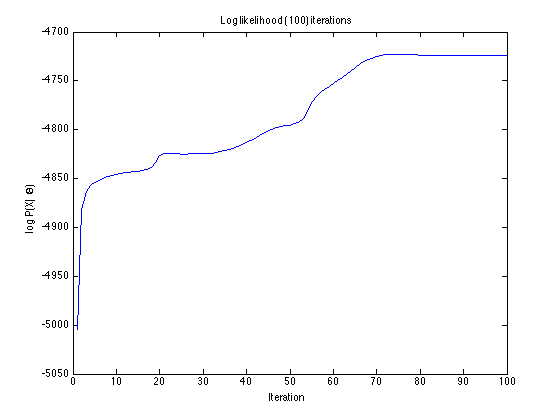
\includegraphics[scale=.57]{images/log_likelihood_scores.png}
  \caption{Log likelihood scores for case \textbf{a}}
  \label{fig:log_likelihood_a}
\end{figure}

To see the effect of EM algorithm visually we assign each data point to one of the four clusters $k = 1,2,3,4$ using the maximum posterior probability rule then plot three separate graphs for $t = 10,50,100$.

$$ k^* = \argmax_{1 \le k \le 4} P(z_n=k|x_n;\Theta^{(t)}) $$

\begin{figure}[H]
  \centering
    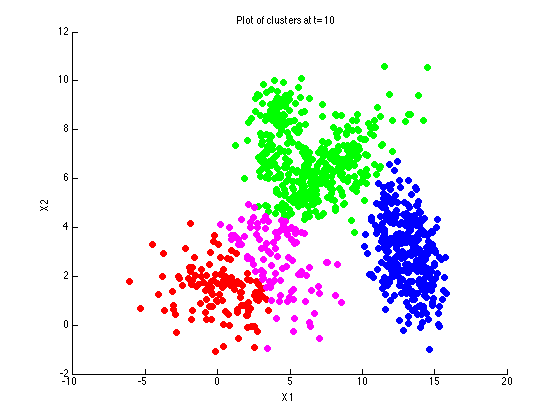
\includegraphics[scale=.57]{images/clusters_t_10.png}
  \caption{Plot of the four clusters at t=10}
\end{figure}

\begin{figure}[H]
  \centering
    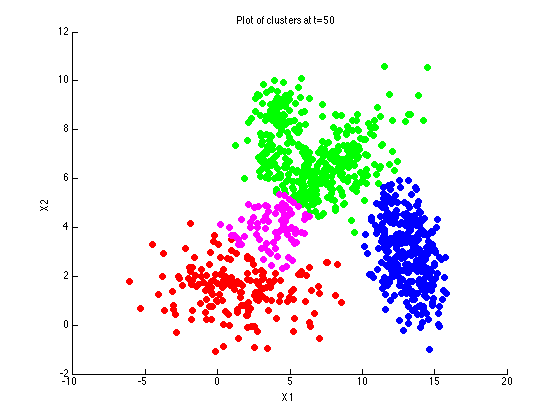
\includegraphics[scale=.57]{images/clusters_t_50.png}
  \caption{Plot of the four clusters at t=50}
\end{figure}

\begin{figure}[H]
  \centering
    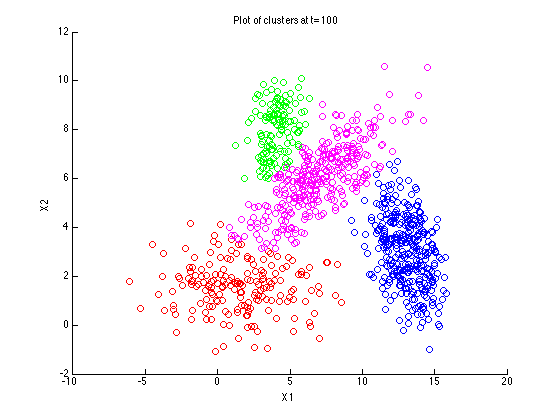
\includegraphics[scale=.57]{images/clusters_t_100.png}
  \caption{Plot of the four clusters at t=100}
\end{figure}

\newpage
\subsection*{Appendix:}
	\lstinputlisting[language=Matlab, title=\lstname, basicstyle=\footnotesize]{problem_1.m}
	\lstinputlisting[language=Matlab, title=\lstname, basicstyle=\footnotesize]{EM.m}
	\lstinputlisting[language=Matlab, title=\lstname, basicstyle=\footnotesize]{gamma_nk.m}
	\lstinputlisting[language=Matlab, title=\lstname, basicstyle=\footnotesize]{mvnpdf.m}
\end{document}